\documentclass[25pt, a0paper, landscape]{tikzposter}
\tikzposterlatexaffectionproofoff
\usepackage[utf8]{inputenc}
\usepackage{authblk}
\makeatletter
\renewcommand\maketitle{\AB@maketitle} % revert \maketitle to its old definition
\renewcommand\AB@affilsepx{\quad\protect\Affilfont} % put affiliations into one line
\makeatother
\renewcommand\Affilfont{\Large} % set font for affiliations
\usepackage{amsmath, amsfonts, amssymb}
\usepackage{tikz}
\usepackage{pgfplots}
% align columns of tikzposter; needs two compilations
\usepackage[colalign]{column_aligned}

% tikzposter meta settings
\usetheme{Default}
\usetitlestyle{Default}
\useblockstyle{Default}

%%%%%%%%%%% redefine title matter to include one logo on each side of the title; adjust with \LogoSep
\makeatletter
\newcommand\insertlogoi[2][]{\def\@insertlogoi{\includegraphics[#1]{#2}}}
\newcommand\insertlogoii[2][]{\def\@insertlogoii{\includegraphics[#1]{#2}}}
\newlength\LogoSep
\setlength\LogoSep{-70pt}

\renewcommand\maketitle[1][]{  % #1 keys
    \normalsize
    \setkeys{title}{#1}
    % Title dummy to get title height
    \node[inner sep=\TP@titleinnersep, line width=\TP@titlelinewidth, anchor=north, minimum width=\TP@visibletextwidth-2\TP@titleinnersep]
    (TP@title) at ($(0, 0.5\textheight-\TP@titletotopverticalspace)$) {\parbox{\TP@titlewidth-2\TP@titleinnersep}{\TP@maketitle}};
    \draw let \p1 = ($(TP@title.north)-(TP@title.south)$) in node {
        \setlength{\TP@titleheight}{\y1}
        \setlength{\titleheight}{\y1}
        \global\TP@titleheight=\TP@titleheight
        \global\titleheight=\titleheight
    };

    % Compute title position
    \setlength{\titleposleft}{-0.5\titlewidth}
    \setlength{\titleposright}{\titleposleft+\titlewidth}
    \setlength{\titlepostop}{0.5\textheight-\TP@titletotopverticalspace}
    \setlength{\titleposbottom}{\titlepostop-\titleheight}

    % Title style (background)
    \TP@titlestyle

    % Title node
    \node[inner sep=\TP@titleinnersep, line width=\TP@titlelinewidth, anchor=north, minimum width=\TP@visibletextwidth-2\TP@titleinnersep]
    at (0,0.5\textheight-\TP@titletotopverticalspace)
    (title)
    {\parbox{\TP@titlewidth-2\TP@titleinnersep}{\TP@maketitle}};

    \node[inner sep=0pt,anchor=west] 
    at ([xshift=-\LogoSep]title.west)
    {\@insertlogoi};

    \node[inner sep=0pt,anchor=east] 
    at ([xshift=\LogoSep]title.east)
    {\@insertlogoii};

    % Settings for blocks
    \normalsize
    \setlength{\TP@blocktop}{\titleposbottom-\TP@titletoblockverticalspace}
}
\makeatother
%%%%%%%%%%%%%%%%%%%%%%%%%%%%%%%%%%%%%


% color handling
\definecolor{TumBlue}{cmyk}{1,0.43,0,0}
\colorlet{blocktitlebgcolor}{TumBlue}
\colorlet{backgroundcolor}{white}

% title matter
\title{DL4CV Project}

\author[1]{Strobel Maximilian}
\author[1]{Werhahn Maximilian}
\author[1]{Kiener Martin}
\author[1]{Seferis Emmanouil}

\affil[1]{Technical University of Munich}

\insertlogoi[width=15cm]{tum_logo}
\insertlogoii[width=15cm]{tum_logo}

% main document
\begin{document}

\maketitle

\begin{columns}
    \column{0.3}
    \block{Our Idea}{
    For this project we tried adapting already existing methods of reinforcement learning for Atari
    2600 games to train a new architecture to play two Atari games simultaniously only using the same
    action for both. Before coming up with a new architecture we first trained a Deep-Q-Learning neural
    network on multiple single games. For the game Breakout we achieved above human-performance with this
    trained model which was our first goal of this project. After finishing this task we tried various
    new architectures to reach our second goal; to perform better than random play on two Atari games
    concurrently with the same action sequence. 
    }
    \block{Preprocessing \& Environment}{
    	The environment for the learning agents was OpenAI gym. This toolkit for
    	developing and comparing reinforcement learning agents was used as an interface to Atari 2600
    	games like Breakout or SpaceInvaders, that the agents tried to learn. The interface provides
    	informations about the state of the games as well as the current screen. Due to an internal
    	flickering of the games (e.g. shoots are only on odd frames visible), the current screen is
    	obtained by a maximum operation on two successive frames.
    	Before the screen was fed into the neural network with the screen, it was preprocessed as 	
    	depicted in the graphic below.
		\begin{tikzpicture}
		\node[inner sep=0pt] (preprocessing) at (0,0)
    	{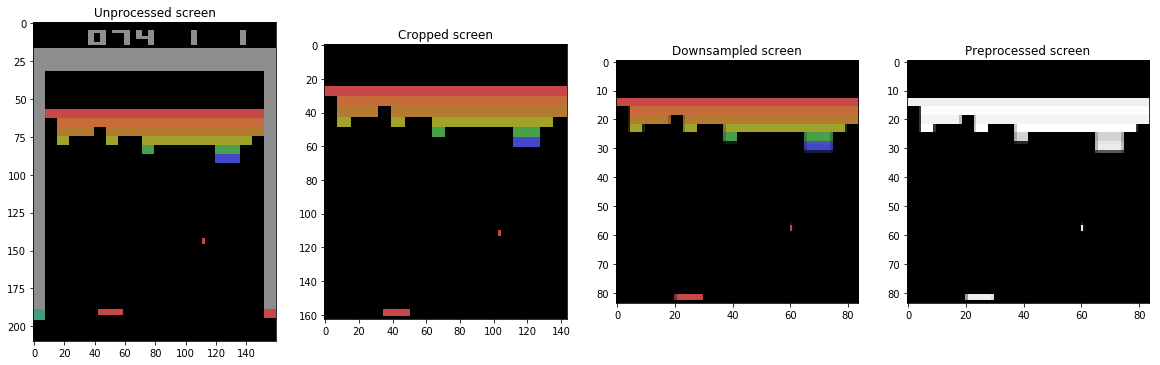
\includegraphics[width=.26\textwidth]{preprocessing_pipeline.png}};
    	\end{tikzpicture}
    	In OpenAI gym there exists a frame skipping technique, that was also modified. Instead of
    	skipping randomly between two and four frames, the frame skipping rate was set to a constant
    	value. During the training the rewards were clamped to -1 and 1 to gain comparability between
    	different games. Additional the loss of one live was punished with a reward of -1, whatever
    	the real reward was.
    }

    \column{0.4}
    \block{First Architecture}{
    	\begin{tikzpicture}
		\node[inner sep=0pt] (Architecture1) at (0,0)
    	{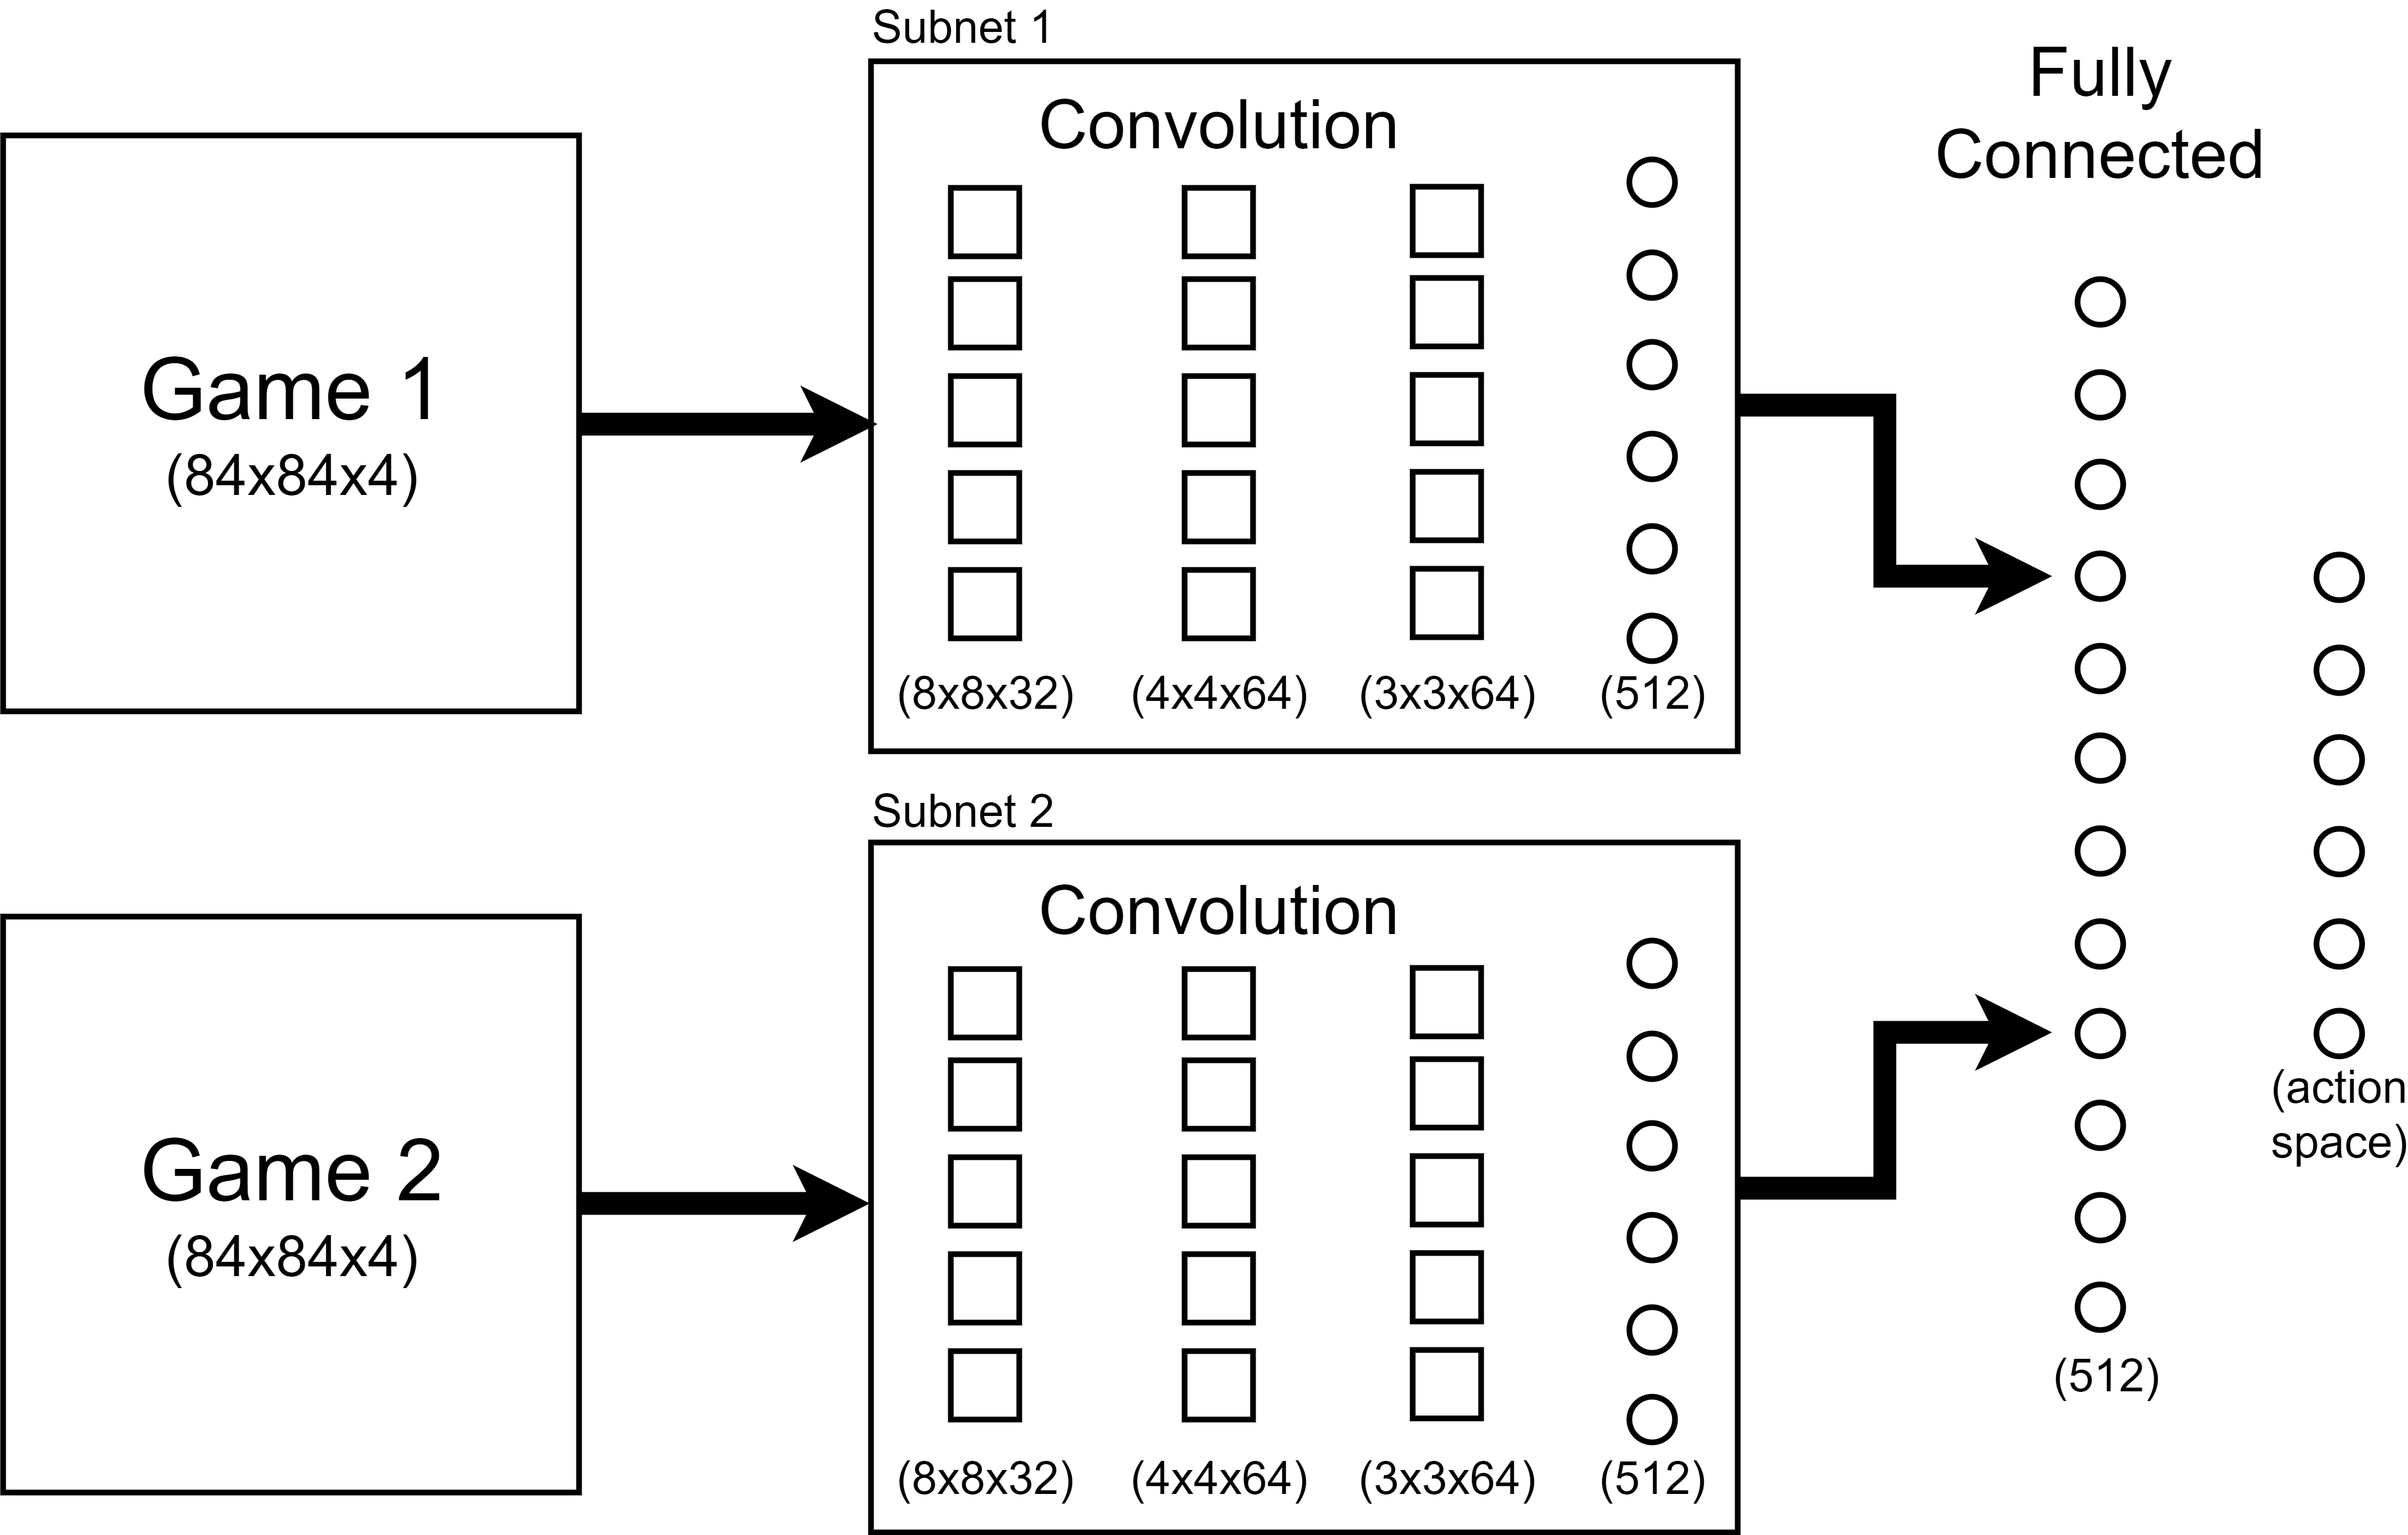
\includegraphics[width=.26\textwidth]{two_nets.png}};
    	\end{tikzpicture}
		For the first architecture we duplicated the already existing DQN model, removed the output
		layers of both subnets and added two additional fully connected layers of size 512 and the
		maximum of the action spaces of the games to map the input screens of both games to one single
		action. Each of the two preprocessed frame histories is fed into one of the subnets separately.
		The resulting output action is then again mapped onto a second action which is used for the other
		game. With this version we already achieved our first goal which is being better than random play.
	}
    \block{Second Architecture}{\begin{tikzpicture}
		\node[inner sep=0pt] (Architecture2) at (0,0)
    	{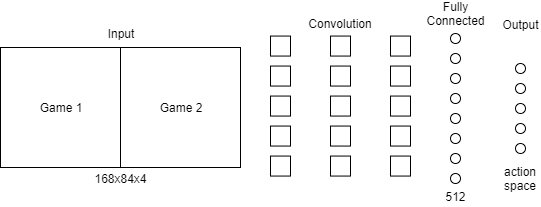
\includegraphics[width=.26\textwidth]{one_net.png}};
    	\end{tikzpicture}
		Another architecture we used to train both games at the same time was the typical DQN model. As
		input the frames of both games were concatenated into a single tensor. The dimensions of the torch
		tensor as input for the DQN is [1,4,168,84]. Furthermore the rewards of both environments are
		combined. The results for this architecture were way worse than for the first architecture.
		(Possible reasons?)
		(More details about the rewards etc.?)
	}

    \column{0.3}
    \block{Visualization}{   
    	\begin{tikzpicture}
		\node[inner sep=0pt] (filter_breakout) at (0,0)
    	{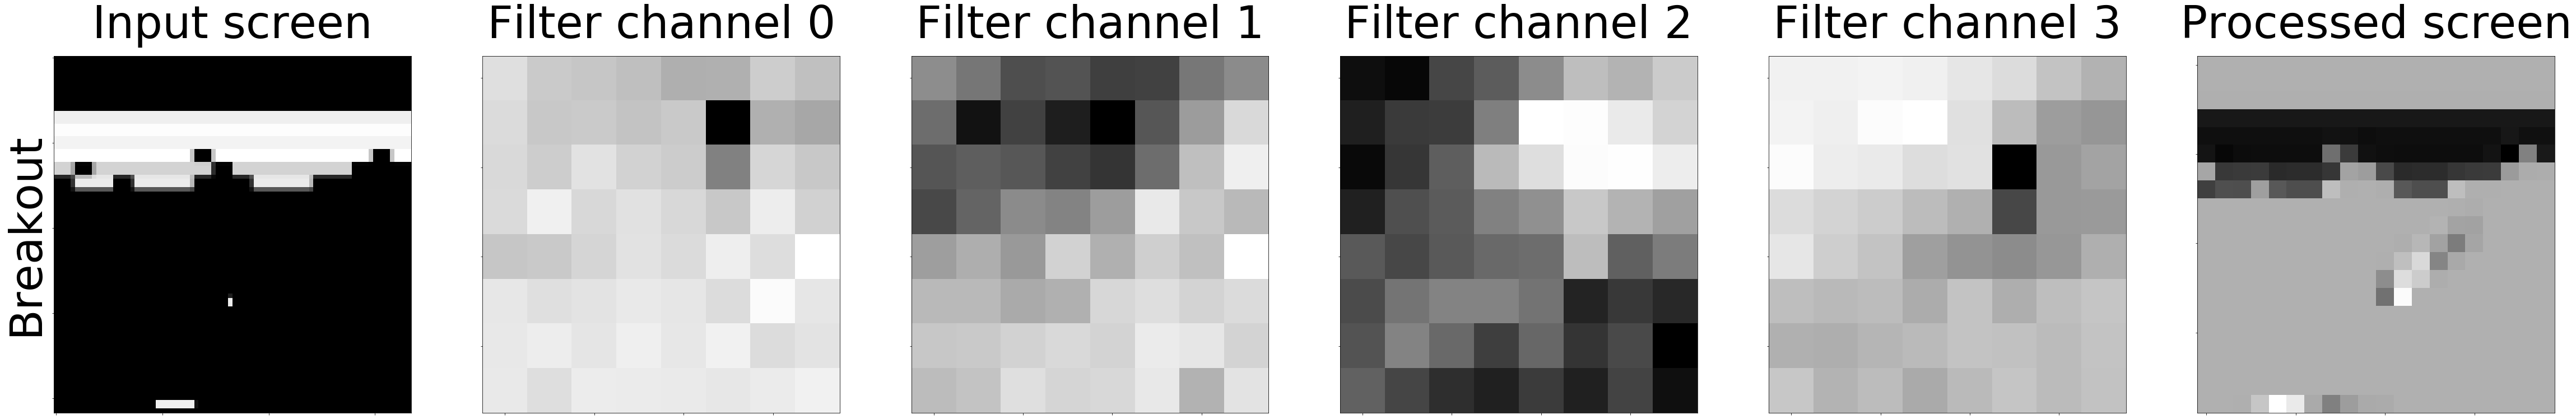
\includegraphics[width=.26\textwidth]{filter_breakout.png}};
    	\end{tikzpicture}
    	\begin{tikzpicture}
		\node[inner sep=0pt] (filter_breakout) at (0,0)
    	{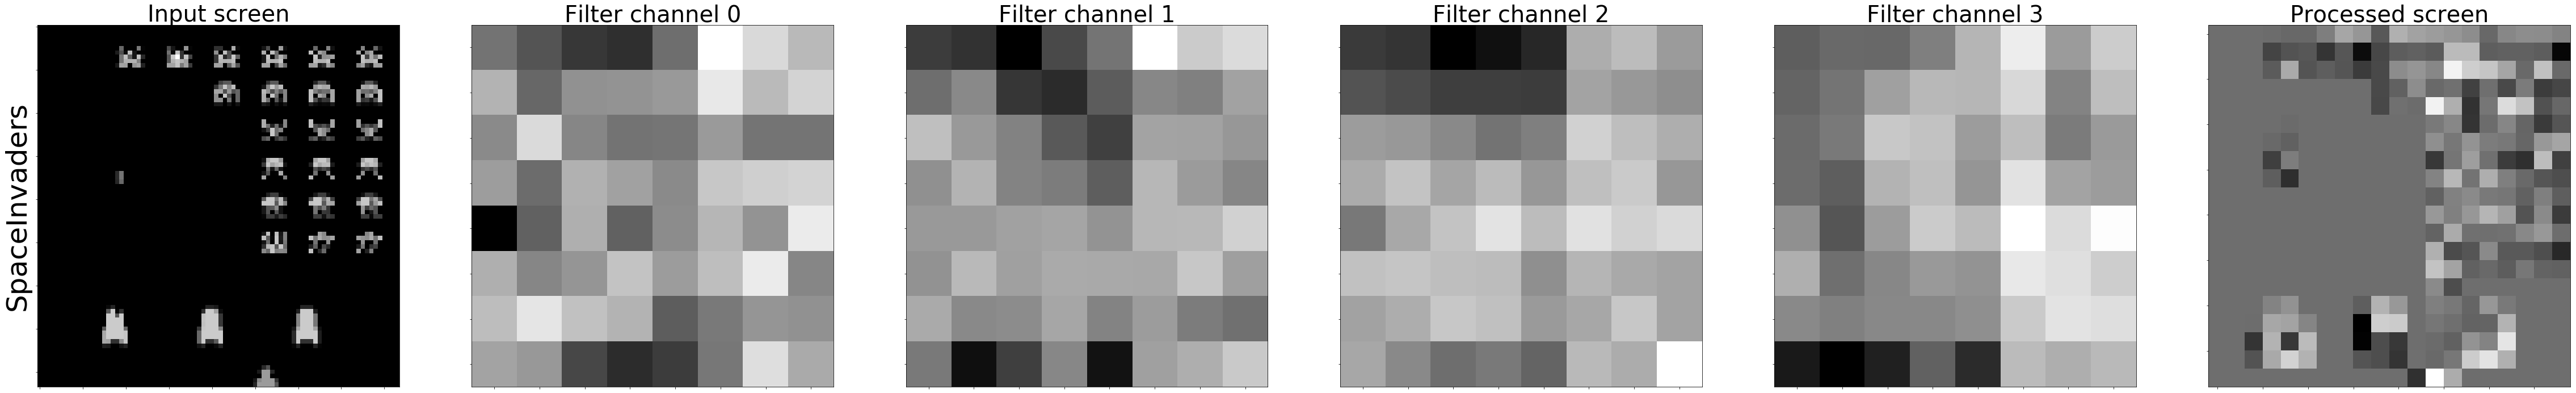
\includegraphics[width=.26\textwidth]{filter_spaceinvaders.png}};
    	\end{tikzpicture}
   	}   	
    \block{Results}{
        \begin{tikzpicture}
		\node[inner sep=0pt] (training) at (0,0)
    	{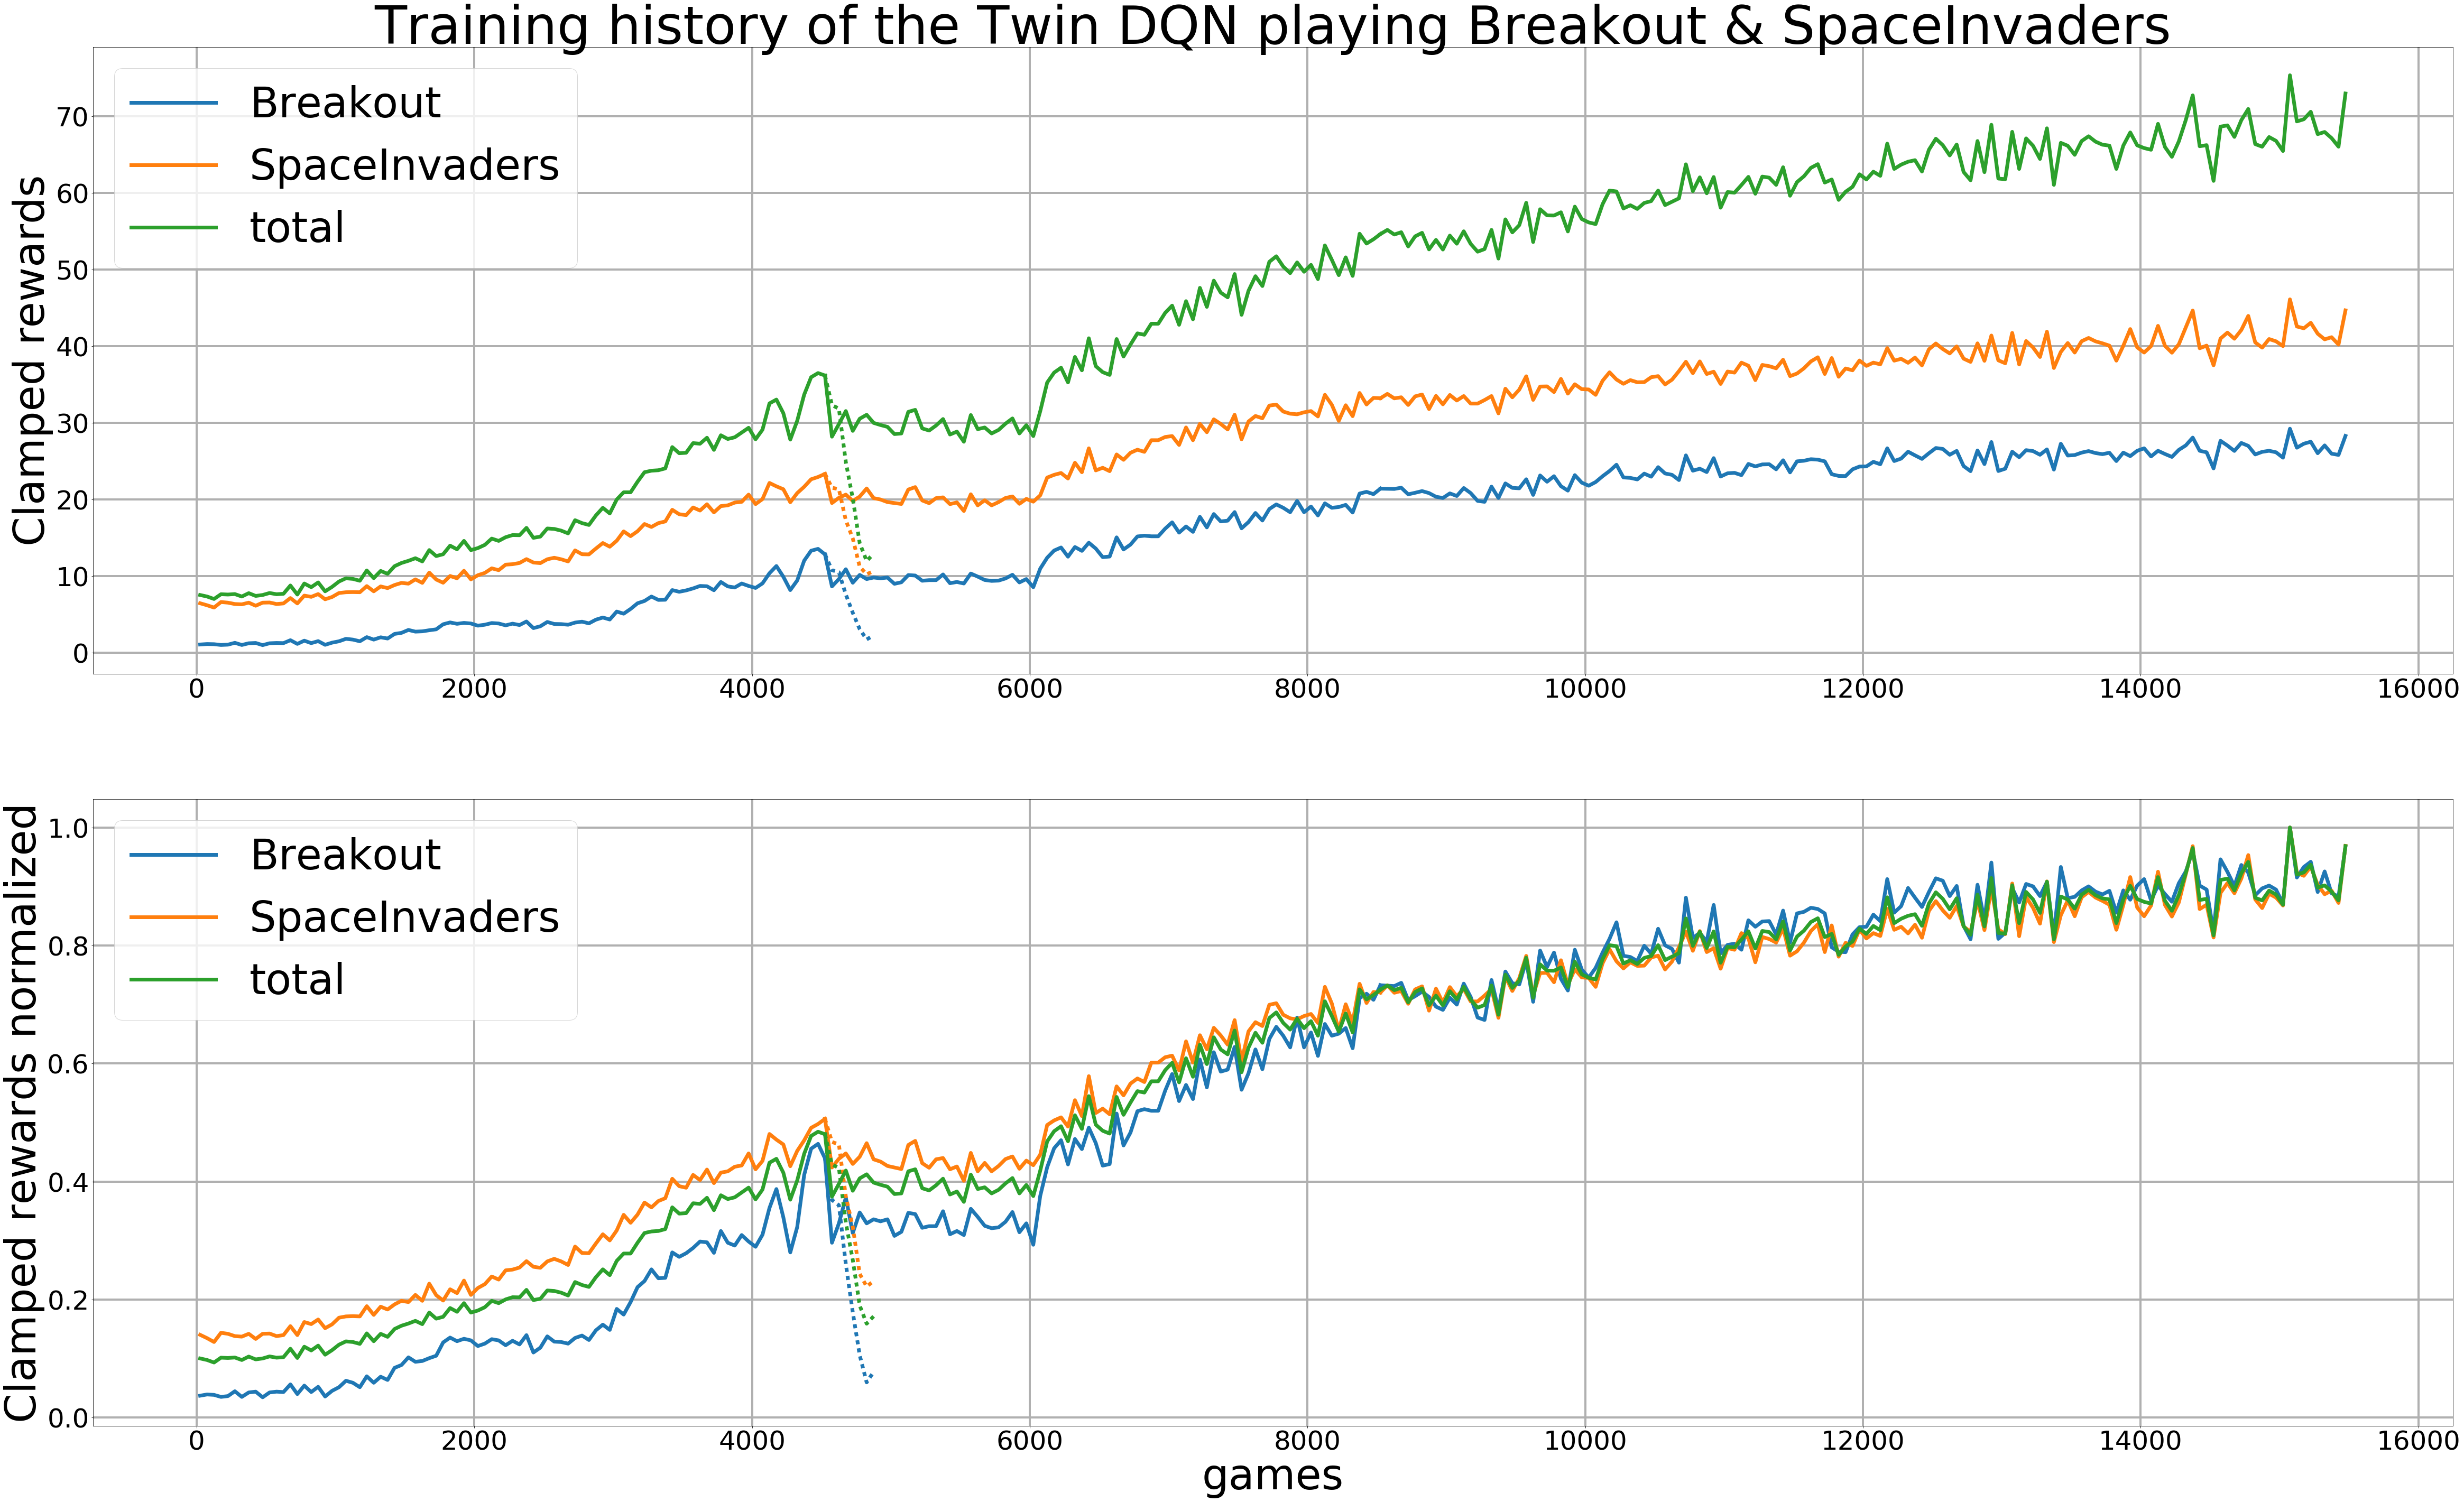
\includegraphics[width=.26\textwidth]{training.png}};
    	\end{tikzpicture}
		\begin{tabular}{ l | c c c}
	 		Games & Random Play & Double DQN & Single DQN  \\
			\hline
			Breakout + SpaceInvaders & (6.9, 40.3) &  (,) & (,)\\
			Phoenix + SpaceInvaders & (24.9, 640.5) & (46.6, 1877.8) & (,)\\
		\end{tabular}
		\\
		The first element of the tuple is the clamped reward which was used for training, second one the
		actual, unclamped reward of both games. The random rewards were averaged over 20000 episodes while the
		rewards for the double DQN took around 3 million steps. It is quite hard to compare these results to
		human performance since there are no records of humans playing two games simultaniously with just one
		controller.
	}
\end{columns}

\end{document}
